\clearpage
\section{远处铁丝的取样}
近看一根铁丝，它能占好几个像素，每个像素大致可以判断为铁丝或背景。镜头拉远后，一个像素可能同时盖住铁丝和后面的墙。要比较两种画法，可以先算铁丝在每个像素内实际占了多大面积。若铁丝挡住四分之一，这个像素的颜色也应保留后面四分之三的墙面。

\begin{figure}[H]\centering
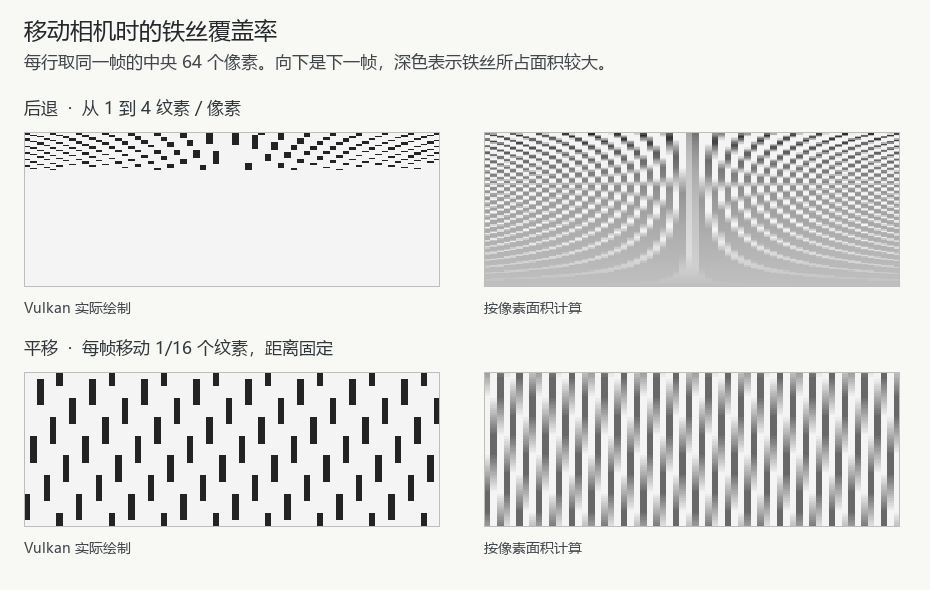
\includegraphics[width=.82\linewidth]{../../../output/validation/fine-mask-motion/motion.png}
\caption{左列是加入 SSAA 前的 Vulkan 单点绘制，右列按同一相机位置计算面积。每一行是该帧画面中央的一排像素，向下读就是镜头的运动过程。后退时左上图变成整片浅色，说明渲染丢掉了铁丝。测试所用引擎库的 SHA-256 以 \texttt{36d47099} 开头。}
\end{figure}

相机不动时，连续 8 帧逐像素相同。让相机每帧横移相当于原图十六分之一列的距离，铁丝在画面中仍应平均占 25\% 的面积。正式绘制却在 12.5\% 和 25\% 之间跳了 16 次。其中相邻两帧有 512 个像素一起从空隙变为铁丝。在另一次缓慢后退的测试里，从一个屏幕像素横跨 1.75 个纹素起，铁丝连续 91 帧消失。拾取轮廓与绘制轮廓始终一致，问题出在两者共用的材质裁剪。\href{run:../validation/fine-mask-motion/report.json}{195 帧的实测}\quad\href{run:../validation/fine-mask-motion/frames.csv}{逐帧数据}

我们试算了另一种选择。在每个像素覆盖的区域内固定选一个点，读取原图的透明度。这样铁丝不会在缩图时被抹掉。在一个像素横跨 26.51 个纹素的固定机位上，这个办法让铁丝占到 25.83\%，接近面积参考的 24.98\%。但放大单个像素看，它仍然只有完全遮挡和完全透光两种结果。整块网的面积接近了，画面里却多出了黑白颗粒。\href{run:../validation/fine-mask/coverage-candidate.png}{三种取样结果对照}

同一个 CPU 实验把纹理图案横移八分之一个屏幕像素，轮廓和相机保持原位。实际面积在每个像素中平均只变化了约 1.28 个百分点，单点取样却让 35.32\% 的像素直接换色。这个候选保留下来作对照。改用同一帧的多个样本后，仍可沿同一条相机轨迹比较铁丝和墙各占多少，以及相邻帧的颜色变了多少。\href{run:../validation/fine-mask/coverage-candidate.json}{候选计算与取样位置}\quad\href{https://research.nvidia.com/publication/2017-02_hashed-alpha-testing}{Wyman 和 McGuire，I3D 2017}

\clearpage
\subsection{一个像素里的两种表面}
铁丝前面有灯，后面是一堵暗墙。放大两者交界的一个像素，其中四分之一是铁丝，余下的部分透过网孔看见墙。假设铁丝着色后红通道的线性值为 $4.0$，墙为 $0.2$。线性值与收到的光量成正比，这个像素的红色应当是多少？

\begin{figure}[H]\centering
\begin{tikzpicture}[font=\small,x=1cm,y=1cm]
\definecolor{samplewall}{HTML}{DEF1F1}
\definecolor{samplewire}{HTML}{F4CAA0}
\begin{scope}
  \fill[samplewall] (0,0) rectangle (2.5,2.5);
  \fill[samplewire] (0,2.5) -- (0,1.25) -- (2.5,2.5) -- cycle;
  \draw[line] (0,1.25) -- (2.5,1.25) (1.25,0) -- (1.25,2.5);
  \draw[ink] (0,0) rectangle (2.5,2.5);
  \foreach \x/\y in {.625/.625,.625/1.875,1.875/.625,1.875/1.875}
    \fill[ink] (\x,\y) circle (2.4pt);
\end{scope}
\node[align=left,anchor=west,text width=9.5cm] at (3.0,1.25) {\textbf{把一个像素放大看}\\[4pt]
橙色是铁丝的边缘，浅蓝色是后面的墙。四个点各代表同样大的取样区域。一个点看见铁丝，另外三个点分别看见墙。};
\end{tikzpicture}
\caption{项目绘制的面积示意。图中铁丝占据像素四分之一的面积，四点估计碰巧与它相等。铁丝再偏一点，四个点数出的比例可能与实际面积有差别。}
\end{figure}

把屏幕上的这个像素均分为四份，各画一次深度和材质，灯光就能照到各自可见的表面。最后将四份的颜色相加，再除以四。图中的红通道得到
\[
  L_{\mathrm{red}}=\frac{4.0+0.2+0.2+0.2}{4}=1.15.
\]
绿色和蓝色也这样计算。场景面板用 $0$ 到 $1$ 表示从黑到白，计算光照的图像却需要保留 $4.0$ 这个亮度。若先把四个数各自截到 $1$，再平均，就只得到 $0.4$。Redflag 把亮部压到可显示范围的处理称为色调映射，安排在颜色平均之后。像素覆盖面积与滤波权重的推导见 \source{https://www.pbr-book.org/4ed/Sampling_and_Reconstruction/Image_Reconstruction}{PBRT 第四版，§8.8}。

Redflag 的延迟渲染先为每个取样位置保存可见表面，再计算光照。\path{Redflag/src/Platform/Vulkan/Shaders/Mesh.frag} 将底色、粗糙度和法线写入场景图，同目录的 \path{PackSurfaces.comp} 用该点的深度还原空间位置。把铁丝和墙的深度先平均，会把光照位置放到两者之间的空处。取样位置各自通过深度测试，光照算完后才有四个可以相加的颜色。Intel 在 SIGGRAPH 2010 的课程里把样本分开处理。普通表面只算一次光照，在同一像素出现不同表面的边缘才逐样本着色。这是今后可以用来比较开销的一种办法。\source{https://www.intel.com/content/www/us/en/developer/articles/technical/deferred-rendering-for-current-and-future-rendering-pipelines.html}{Lauritzen，Deferred Rendering for Current and Future Rendering Pipelines}

Vulkan 编辑器开启 \code{SSAA 2×2} 后，\path{RedflagForge/src/LightingPreview.cpp} 的 \code{Render} 把光照图的宽和高各扩大一倍。几何、着色、屏幕效果仍按原来的顺序执行，内部光照图现在有四倍的像素要算。最终面板保持原来的像素数。下段是面板显示着色器的简化写法，\code{nextRow} 是放大后的图宽。拾取单独绘制一张实体编号图，沿用原来的相机和裁剪，不会对四个物体编号取平均。

\begin{verbatim}
// 伪代码，i 对应每组四个位置的第一项。颜色按行存放。
red = (light[i].r         + light[i + 1].r
     + light[i + nextRow].r + light[i + nextRow + 1].r) / 4;
// 亮度先压到可显示范围，再换成面板所用的显示值。
panelRed = pow(red / (1 + red), 1.0 / 2.2);
\end{verbatim}
\loc{RedflagForge/src/Shaders/LightingPreview.comp}

\clearpage
\subsection{一张黑白铁丝图缩小以后}
试验原图的每四列有一列白色铁丝，另外三列为黑色网孔。四列缩到一个纹素，就留下约 $0.25$ 的灰色。若照近处的方式把这个值与 $0.5$ 比较，四个取样位置都会落到网孔。单靠把光照图画大，仍然可能整片漏掉远处的网。Yüksel 在 I3D 2018 的文章里展示了胡须随镜头拉远而变稀的对照图，作者的方法在预处理缩小贴图时重新分配透明度。Redflag 保留原贴图，在绘制时决定每个样本是否通过。\source{https://www.cemyuksel.com/research/alphadistribution/}{Yüksel，Alpha Distribution for Alpha Testing}

\begin{figure}[H]\centering
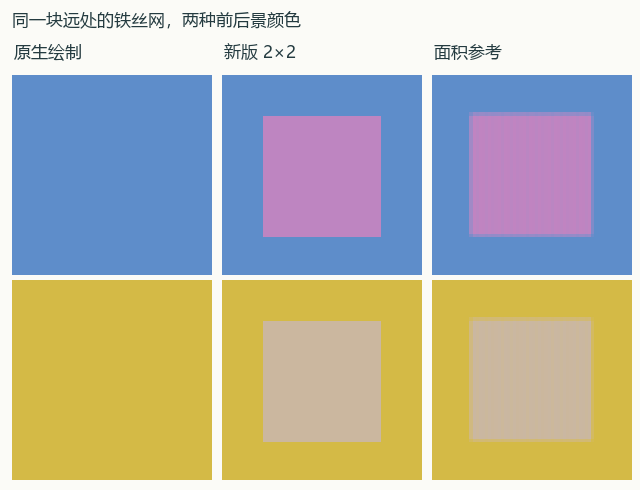
\includegraphics[width=.58\linewidth]{../../../output/validation/mask-supersampling-current/two-colors.png}
\caption{同一个网格，两组自发光材质。每个面板像素横跨原图 26.5 列。左列是单点绘制，看不见铁丝。中列是四点绘制，能看到前后景混出的颜色。右列用每个像素里实心部分的实际宽度计算，网格边缘和内部仍有细微明暗变化。前两列来自 Vulkan 读回，三列使用同一显示转换。}
\end{figure}

在原图上，白色是铁丝，黑色是网孔。镜头拉远时，先读出一个面板像素里四个位置的灰度，再用平均灰度估计铁丝所占的面积。例如四个位置分别读到 $0.95,0.45,0.40,0.20$，平均为 $0.50$，应留下两个位置。先留灰度最大的两处，铁丝的轮廓就能跟着纹理走。四处读数完全相同时才用固定顺序。

每个像素只能留下零到四个样本，能表示的面积比例相隔四分之一。因此四个通过值选在每两档的中间，即 $1/8,3/8,5/8,7/8$。平均灰度为 $0.25$ 时只过第一档，留下的那个样本看见铁丝，其余三个看见墙。近处仍按每处自己的灰度与 $0.5$ 比较。屏幕像素从覆盖一个原图纹素逐渐变成覆盖两个纹素时，着色器逐渐转用四处平均和排序。正式代码在 \path{Shaders/Cutout.glsl} 的 \code{coversArea}。

这条规则只用于一种可以从贴图本身确认的材质。底色图的透明度或独立透明图的红通道，须有一张只含黑和白，另一张处处为白。设这次绘制传给着色器的透明度系数为 $a>0$，材质的裁剪值还须恰好是 $a/2$。一般灰度图或不同裁剪值仍直接比较完整的透明度。若两张纹理都决定网孔的位置，单看各自的平均数会弄错图形。比如一张只让左半边通过，另一张只让右半边通过，两张相乘后处处为黑，而两个平均值相乘却是 $0.25$。实际条件见 \path{Redflag/src/Platform/Vulkan/VulkanDraw.cpp} 的 \code{DrawIndexed}，透明度比较在同目录的 \path{Shaders/Cutout.glsl}。

两张网在同一个像素内重叠时，缩图还会丢掉前后两层的相对位置。把两张网叠放，每张各挡四分之一；将后面那张的花纹平移两列，真实的两组铁丝合计遮住一半。缩小后，两张图都给出 $0.25$，于是两层网挑中同一个取样位置。这次 GPU 实测只留下四分之一的铁丝。深度测试仍能选对每个位置前面的那层，没保留下来的是两层铁丝在像素中原本错开的距离。\href{run:../validation/mask-supersampling/subpixel-materials.csv}{单层与两层网的 Vulkan 读回}

Vulkan 也提供由透明度决定多个样本是否保留的功能（alpha-to-coverage），规范读取的是第一个颜色输出中的 alpha。Redflag 的这一个值存着粗糙度和金属度，还用符号区分发光表面。为保留现有材质数据，编辑器直接在放大的光照图上取样。\source{https://docs.vulkan.org/spec/latest/chapters/fragops.html\#fragops-covg}{Khronos，Fragment Operations，Multisample Coverage}

\clearpage
\subsection{移动镜头时的铁丝颜色}
铁丝和背板分别用固定的颜色发光。假设某一帧、某个像素里铁丝占比为 $p$，用铁丝颜色乘以 $p$，再加上墙的颜色乘以 $1-p$，就得到该像素的参照颜色。$p$ 可以直接由镜头位置和铁丝在原图中的宽度算出。测试将两组前后景颜色交换明暗并改变色相，分别用 Vulkan 绘制，再读取 $64\times64$ 幅面的线性 RGB。图中每列除了最右侧的数学参照，都是 GPU 的结果。

\begin{figure}[H]\centering
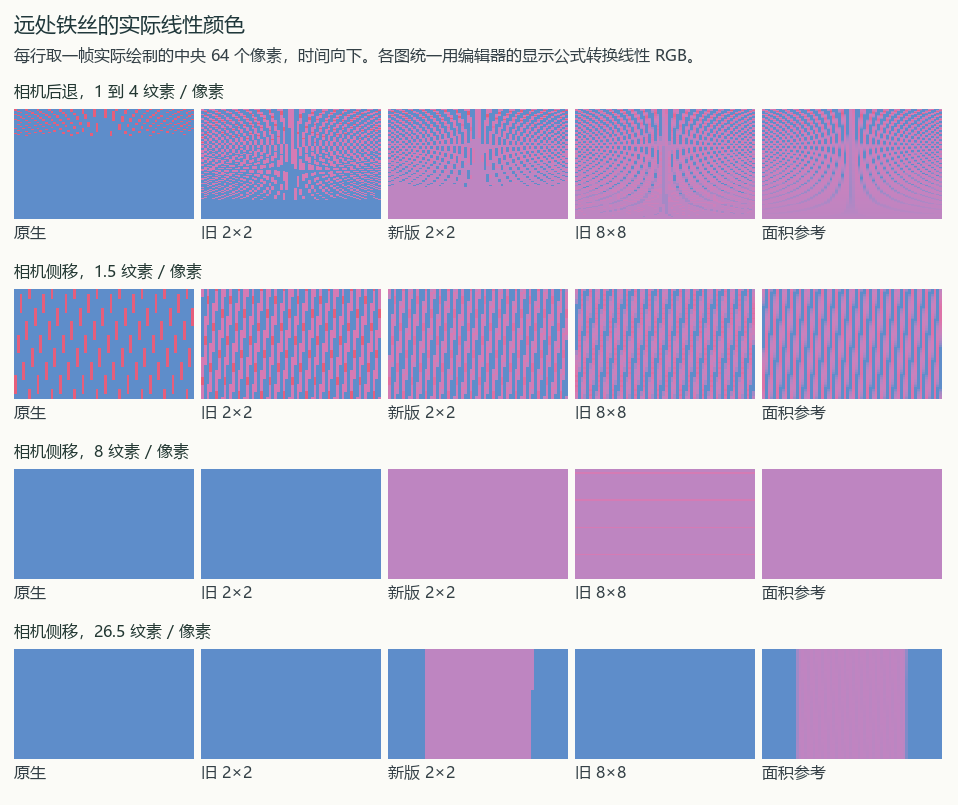
\includegraphics[width=.94\linewidth,trim=0 373bp 0 0,clip]{../../../output/validation/mask-supersampling-current/motion.png}
\caption{每幅图里，时间都从上往下读。上排让相机缓慢后退，下排让相机水平移动。图中的“旧 $2\times2$”和“旧 $8\times8$”仅提高分辨率，每个位置仍一律按 $0.5$ 裁剪。对照最右侧的实际面积，上排第一幅有大片帧只剩蓝底，第三幅还能看见铁丝。\href{run:../validation/mask-supersampling-current/motion.png}{查看含两组远景的完整实测图}}
\end{figure}

比较闪动，要扣除相机真的移动所产生的变化。比如原图预测某一像素的铁丝从占 20\% 变为 22\%，绘制却从完全空变成四分之一实心，那么这次绘制多跳了 $25-2=23$ 个百分点。把这种差的绝对值对每个像素、每对相邻帧取平均，得到“变化误差”。另一个指标“覆盖误差”直接比较每个像素里画出的比例与实际面积。这两项分别回答画面跳了多少、铁丝占得准不准。\href{run:../validation/mask-supersampling-current/frames.csv}{各帧机位和误差}\quad\href{run:../validation/mask-supersampling-current/report.json}{设备、程序与 GPU 读回}

{\small\noindent\begin{tabularx}{\linewidth}{@{}Yrrr@{}}\toprule
竖铁丝，误差单位为百分点 & 单点 & 初版四点 & 四点按灰度排序 \\\midrule
镜头后退，覆盖误差 & 23.29 & 8.56 & 5.44 \\
镜头后退，变化误差 & 9.90 & 10.59 & 5.54 \\
镜头平移，覆盖误差 & 20.06 & 9.13 & 5.32 \\
镜头平移，变化误差 & 5.08 & 4.95 & 3.91 \\\bottomrule
\end{tabularx}\par}

后退的 121 帧里，单点绘制末尾连续 91 帧只剩背景。表中的“初版四点”给四个位置各分配一个固定的通过值，保住了网，变化误差却比单点还高。让四个位置共用面积估计，再优先留下最接近铁丝的位置，两项误差都降低了。改用斜铁丝，后退时变化误差也从初版四点的 9.24 降到 6.01 个百分点。每像素横跨 26.5 个纹素的远景里，中央区域保有四分之一的铁丝，网格外沿仍能看出四点取样与实际面积的差距。\href{run:../validation/mask-footprint-compare-rank/report.json}{不同方向的逐项实测}

在仓库根目录运行 \path{tests/run_mask_supersampling.cmd} 可重画竖铁丝。\path{tests/MaskSupersampling.cpp} 的 \code{Measure} 为两张自发光方片分别写深度和颜色，再执行显示着色器。测量用 Debug x64 和 RTX 5070 Ti Laptop GPU。对 Sponza 的 $384\times246$ 输出，逐帧着色的位置会从 94,464 增到 377,856。因此编辑器默认关闭 SSAA。整帧时间、显存和 RenderDoc 回放见《渲染性能实测》的“SSAA 的四个着色样点”。\href{run:Redflag-Rendering-Performance.pdf}{渲染性能实测}
